% Name: Loops in the punctured plane
% Description: Two loops based at x₀ in the plane with a point removed: α shrinks to x₀ through the dashed loops, while β winds round the hole and cannot.
% Tags: homotopy, fundamental group, punctured plane, loops, topology

\usetikzlibrary{arrows.meta, decorations.markings}

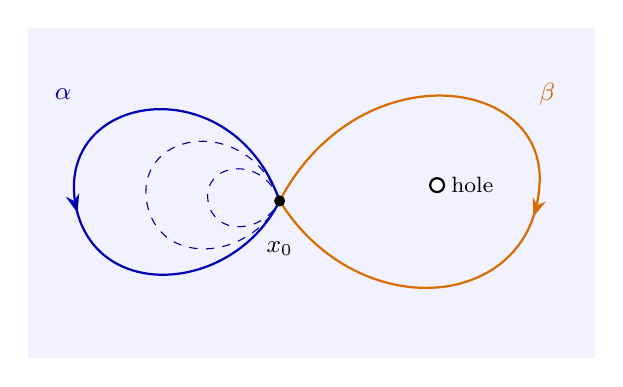
\begin{tikzpicture}[thick, every node/.style={font=\small},
    mid/.style={postaction={decorate}, decoration={markings, mark=at position 0.55 with {\arrow{Stealth}}}}]
  \fill[blue!5] (-3.2,-2) rectangle (4,2.2);
  \coordinate (x0) at (0,0);
  % β goes round the hole at (2, 0.2); α stays left of it, and its dashed copies shrink toward x₀
  \draw[mid, orange!85!black] (x0) .. controls (1,1.9) and (3.4,1.6) .. (3.3,0.2) .. controls (3.2,-1.4) and (1,-1.6) .. (x0);
  \draw[mid, blue!70!black] (x0) .. controls (-0.6,1.7) and (-2.8,1.4) .. (-2.6,0) .. controls (-2.4,-1.3) and (-0.6,-1.2) .. (x0);
  \foreach \s in {0.65, 0.35} \draw[thin, dashed, blue!60!black, scale=\s] (x0) .. controls (-0.6,1.7) and (-2.8,1.4) .. (-2.6,0) .. controls (-2.4,-1.3) and (-0.6,-1.2) .. (x0);
  \draw[fill=white] (2,0.2) circle (2.5pt);
  \node[right, font=\footnotesize] at (2.05,0.2) {hole};
  \fill (x0) circle (2pt) node[below=11pt] {$x_0$};
  \node[blue!70!black] at (-2.75,1.35) {$\alpha$};
  \node[orange!80!black] at (3.4,1.35) {$\beta$};
\end{tikzpicture}
